\begin{figure}
  \centering
  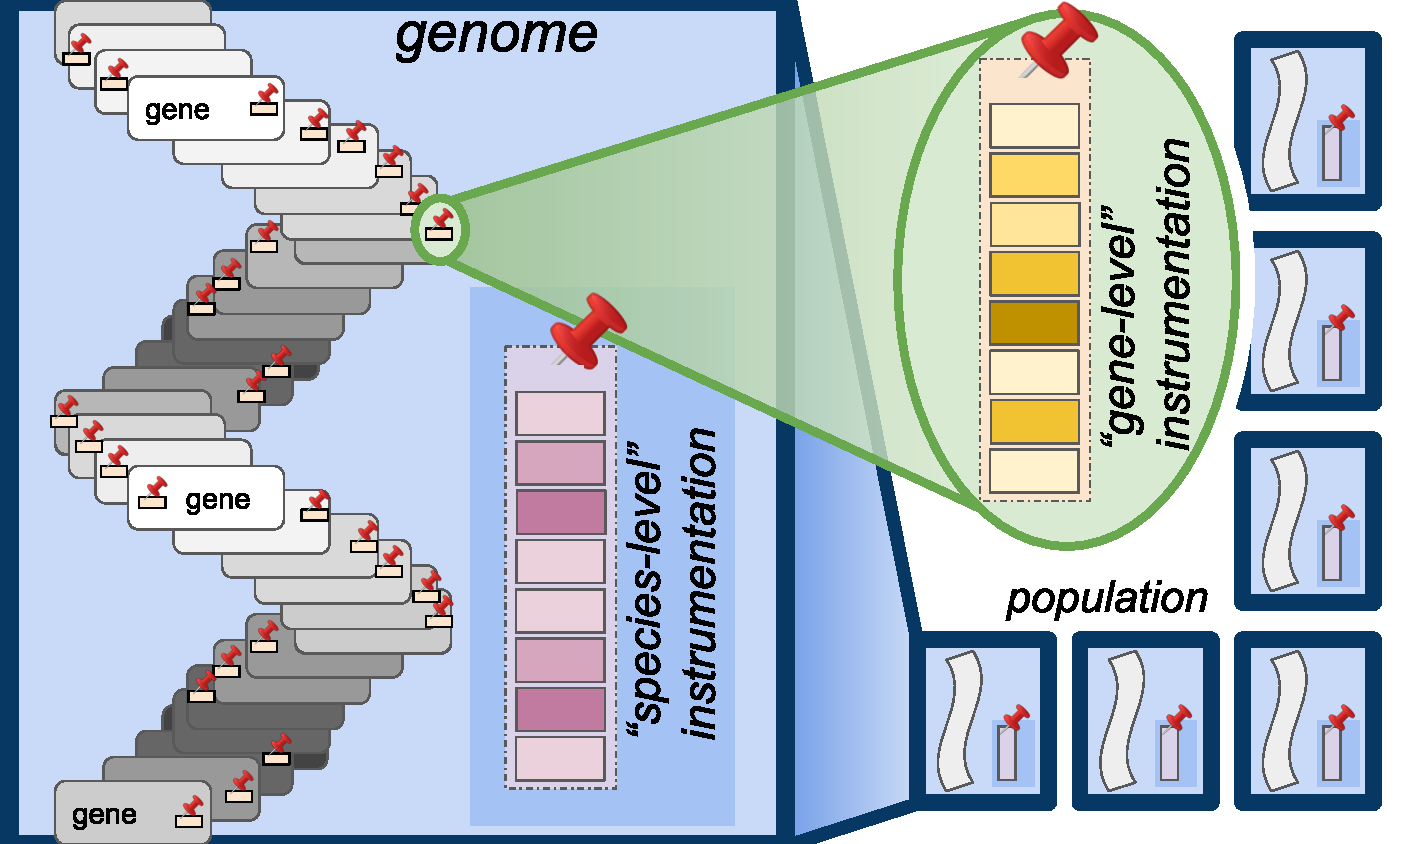
\includegraphics[width=\textwidth]{img/annotation-types}
  \caption{
    Comparison of proposed instrumentation methods: ``species-level'' instrumentation and ``gene-level'' instrumentation.
    Each organism has a single hereditary stratigraph attached as species-level instrumentation, and a gene drive mechanism (Figure \ref{fig:gene-drive}) is used to ensure instrumentation consistency within species (i.e., interbreeding populations).
    Gene-level instrumentation affixes one hereditary stratigraph per gene and can be used for gene tree reconstructions.
    In systems with large number of genes, it may be preferable to attach gene-level instrumentation to a random subset of genes.
  }
  \label{fig:annotation-types}
\end{figure}
